% Document pre-amble
\documentclass{beamer}
\usepackage{mathrsfs, amsthm, amsmath, booktabs, tikz}
\usetheme{CambridgeUS}
\usecolortheme{dove}
\usefonttheme[onlymath]{serif}
\beamertemplatenavigationsymbolsempty{}
\makeatletter
\setbeamertemplate{footline}{}
\makeatother

\title{Semigroups in \textsc{GAP}:\\an introduction and tutorial}
\author{Wilf Wilson\\University of St Andrews}
\date{21 October 2016}

\begin{document}


% Slide: title page
\frame[noframenumbering]{\titlepage}


% Slide: an introduction to transformations, and their use in GAP
\frame{\frametitle{Transformations in \textsc{GAP}}
  A transformation is a function on the set $\{1,\ldots,n\}$. Examples:

  \vspace{0.6em}

  $$f =
  \begin{pmatrix}
    1 & 2 & 3 & 4 & 5 & 6 \\
    4 & 1 & 1 & 5 & 3 & 3
  \end{pmatrix},
  \quad
  g = 
  \begin{pmatrix}
    1 & 2 & 3 & 4 & 5 & 6 \\
    4 & 5 & 1 & 2 & 1 & 4
  \end{pmatrix}.$$

  $$\text{Composition of transformations:}\quad
  fg = \begin{pmatrix}
    1 & 2 & 3 & 4 & 5 & 6 \\
    2 & 4 & 4 & 1 & 1 & 1
  \end{pmatrix}.$$

  \vspace{1em}

  In \textsc{GAP}, a transformation is stored as a list:

  $$f = \text{[ 4, 1, 1, 5, 3, 3 ]},\quad g = \text{[ 4, 5, 1, 2, 1, 4 ]},
  \quad\text{etc.}$$

  \vspace{1em}

  \quad$\texttt{gap> f := Transformation([4, 1, 1, 5, 3, 3]);}$

  \quad$\texttt{gap> S := Semigroup(f);}$
}


% Slide: the definition of a semigroup (mathematically, and in GAP)
\frame{\frametitle{The definition of a semigroup}

  A semigroup is a set $(S)$ with an associative binary operation $(\ast)$.

  \vspace{1em}

  Associativity:\quad $(x \ast y) \ast z = x \ast (y \ast z)$.

  \vspace{1.5em}

  In \textsc{GAP}:
  \quad
  \texttt{IsSemigroup = IsMagma and IsAssociative}.

  In \textsc{GAP}:
  \quad
  \texttt{IsMonoid = IsMagmaWithOne and IsAssociative}.

  In \textsc{GAP}:
  \quad
  \texttt{IsGroup = IsMagmaWithInverses and IsAssociative}.


  \vspace{2.5em}

  We wish to compute with semigroups.
}


% Slide: specifying a semigroup abstractly via a multiplication table
\frame{\frametitle{Specifying a semigroup by multiplication table}

  A finite semigroup can be specified by a multiplication table.  An example:

  \vspace{1em}

  % The following is an example of a multiplication table
  \begin{center}
    \begin{tabular}{c|cccc}
        & 1 & 2 & 3 & 4 \\
      \hline
      1 & 1 & 2 & 3 & 4 \\
      2 & 2 & 1 & 3 & 4 \\
      3 & 3 & 4 & 3 & 4 \\
      4 & 4 & 3 & 3 & 4 \\
    \end{tabular}
  \end{center}
  % End of multiplication table

  \begin{itemize}
    \item
      The row and column labels are the elements.
    \item
      The entry in row $i$, column $j$ defines the product $i \cdot j$.
  \end{itemize}

  \vspace{1.5em}

  Multiplication tables are abstract, but usually impractical.
}


% Slide: table showing numbers of multiplication tables, semigroups, and groups
\frame{\frametitle{An aside: counting multiplication tables}

  % A large table showing the number of n * n tables, where the table defines
  % a magma, a semigroup, or a group.
  \begin{center}
    \begin{tabular}{r|rrrrrr}
        & 1 & 2  & 3      & 4             & $n$ \\
      \hline
      All tables
        & 1 & 16 & 19,683 & 4,294,967,269 & $n^{n^{2}}$ \\
      Magmas
        & 1 & 10 & 3,330  & 178,981,952   & $\sim\!n^{n^{2}}\!/{n\,!}$\\
      Semigroups
        & 1 & 4  & 18     & 126           & \text{?}\\
      Groups
        & 1 & 1  & 1      & 2             & \text{?}\\
    \end{tabular}
  \end{center}

  \vspace{1em}

  There are 12,418,001,077,381,302,684 semigroups of order 10.
}


% Slide: some examples of types of semigroup with natural operations
\frame{\frametitle{Some examples of semigroups}
  Examples:

  \vspace{1em}

  \begin{itemize}
    \item
      Transformations, with composition of functions.
    \item
      Partial permutations, with composition of (partial) functions.
    \item
      $n \times n$ matrices, with matrix multiplication.
    \item
      Finite strings, with concatenation.
    \item
      Binary relations, with composition of relations.
    \item
      Subsets of a set, with union/intersection.
  \end{itemize}

  \vspace{1.5em}

  We can specify such a semigroup with reference only to its elements.
}


% Slide: semigroups defined by a generating set
\frame{\frametitle{Semigroups by generating set}

  A semigroup can be specified by a set of generators.

  The elements are all possible combinations of the generators. Example:
  
  $$(\mathbb{N}, +) = \langle 1 \rangle.$$
  % Natural numbers with addition is generated by the number 1

  \vspace{1em}

  \textbf{Question}:\quad what is a generating set for $(\mathbb{N}, \times)$?
  % Natural numbers with multiplication?
  
  \vspace{2em}

  \textbf{Theme}:\quad we try to compute \emph{without} having to find all the elements.
}


% Slide: basic properties of semigroups for computation
\frame{\frametitle{What might we want to compute?}

  \begin{itemize}
    \item
      Test commutativity.
    \item
      Test membership.
    \item
      Compute the (number of) elements.
    \item
      Count the idempotents.
    \item
      Find the maximal subgroups or subsemigroups.
    \item
      Find the Green's relations.
  \end{itemize}

  \vspace{2em}

  Green's equivalence relations $\mathscr{L}$, $\mathscr{R}$, and $\mathscr{H}$:

  % A list defining Green's L, R, and H relations
  \begin{itemize}
    \item
      $x \mathscr{L} y$ if and only if $x = ay$ and $y = bx$
        \quad(for some $a, b$).
    \item
      $x \mathscr{R} y$ if and only if $x = ya$ and $y = xb$
        \quad(for some $a, b$).
    \item
      $x \mathscr{H} y$ if and only if $x \mathscr{L} y$ and $x \mathscr{R} y$.
  \end{itemize}
}


% Slide: finitely presented semigroups
\frame{\frametitle{Finitely presented semigroups}

  Specify a semigroup by generators and relations. An example:

  $$\langle x, y \ | \ x y = y x,\ 
                       x ^ {3} = x ^ {2},\ 
                       y ^ {2} = y \rangle$$

  \begin{itemize}
    \item
      Works for finite semigroups, and many infinite semigroups.
    \item
      Difficult to write algorithms.
    \item
      Leads to problems of undecidability. 
  \end{itemize}

  \vspace{2em}

  Often, we deal with semigroups that we \emph{know} are finite.
}


% Slide: an algorithm to compute a finite semigroup defined by generators
\frame{\frametitle{Naive exhaustive enumeration of a semigroup}

  Given a set of generators $A$ of a finite semigroup $S$, we can find all the
  elements of $S$ with the following procedure: 

  \vspace{1em}

  % Essential idea: multiply each element by each generator, until nothing new
  % is found.
  \begin{itemize}
    \item
      Define $S = A$.
    \item
      For each $s \in S$, and for each $a \in A$:
      \begin{itemize}
        \item
          if $sa \not\in S$:
          \begin{itemize}
            \item
              add $a$ to $S$.
          \end{itemize}
      \end{itemize}
    \item
      Return $S$ as the set of elements.
  \end{itemize}

  \vspace{2em}

  Requires $|S|\cdot|A|$ multiplications and searches.
}


% Slide: Cayley graphs - a depiction of a right Cayley graph of an unknown semigroup
\frame{\frametitle{}

  The right Cayley graph for $S = \{ x, y, a, b, c \}$; generating set $\{x, y\}$:

  \begin{center}
    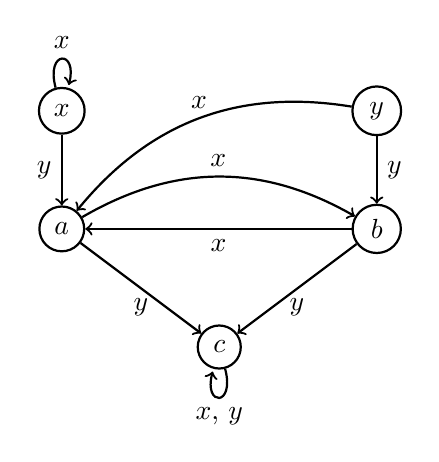
\begin{tikzpicture}[->,thick,elt/.style={circle,draw}]
      \node[elt] (1)  at (0, 3) {$x$};
      \node[elt] (2)  at (4, 3) {$y$};
      \node[elt] (3)  at (0, 1.5) {$a$};
      \node[elt] (4)  at (4, 1.5) {$b$};
      \node[elt] (5)  at (2, 0) {$c$};

      \path
        (1) edge [loop above] node         {$x$} (1)
            edge              node [left]  {$y$} (3)
        (2) edge [bend right] node [above] {$x$} (3)
            edge              node [right] {$y$} (4)
        (3) edge [bend left]  node [above] {$x$} (4)
            edge              node [below] {$y$} (5)
        (4) edge              node [below] {$x$} (3)
            edge              node [below] {$y$} (5)
        (5) edge [loop below] node         {$x$, $y$} (5);
    \end{tikzpicture}
  \end{center}

  \vspace{0.5em}

  Associativity gives us left multiplication: $x(yzt) = (xyz)t$.

  \vspace{0.5em}

  Thus we obtain the left Cayley graph and the Green's relations.
}


% Slide: stating the main mission of computational semigroup theory.
\frame{\frametitle{How can we avoid enumerating the semigroup?}

  A fundamental problem in computational semigroup theory.

  \vspace{2em}

  \begin{itemize}
    \item
      Use the generators.
    \item
      Use theory.
    \item
      Use the representation.
    \item
      Use the power of \textsc{GAP}!
  \end{itemize}
}


% Slide: the definition of a commutative semigroup
\frame{\frametitle{Case study: commutative semigroups}

  \emph{Commutative semigroup}:\quad where $x * y = y * x$ for all $x$ and $y$.

  \vspace{2em}

  How do we test for commutativity?
}


% Slide: the definition of an idempotent in a semigroup
\frame{\frametitle{Case study: counting idempotents}

  An \emph{idempotent}:\quad an element $x$ where $x * x = x$.

  \vspace{1em}

  \begin{itemize}
    \item
      Some semigroups have no idempotents.
    \item
      Some semigroups consist only of idempotents.
    \item
      There exist semigroups at every point between these extremes.
  \end{itemize}

  \vspace{2em}

  How do we count the idempotents in a semigroup?
}


% Slide: pointing out how the properties inherent in the representation of a
% semigroup (e.g. as transformations, say) can give information about the
% semigroup-theoretic properties.
\frame{\frametitle{Using the representation of a semigroup}

  Full transformation semigroup:
  \begin{itemize}
    \item
      $x \mathscr{L} y$ if and only if $\textrm{im}(x) = \textrm{im}(y)$.
    \item
      $x \mathscr{R} y$ if and only if $\ker(x) = \ker(y)$.
  \end{itemize}

  \vspace{1em}

  Full matrix semigroup (over a field):
  \begin{itemize}
    \item
      $x \mathscr{L} y$ if and only if $x$ and $y$ have the same row space.
    \item
      $x \mathscr{R} y$ if and only if $x$ and $y$ have the same column space.
  \end{itemize}

  \vspace{1em}

  Partition monoid:
  \begin{itemize}
    \item
      $x \mathscr{L} y$ if and only if $x^{*}x = y^{*}y$.
    \item
      $x \mathscr{R} y$ if and only if $xx^{*} = yy^{*}$.
  \end{itemize}

  \vspace{1em}
  \ldots
}


% Slide: Explaining how a transformation semigroup acts on the images of its elements
\frame{\frametitle{Using the representation: transformation semigroups}

  A transformation `acts' on \emph{points}: $i \mapsto (i)f$.

  \vspace{0.6em}

  A transformation `acts' on \emph{sets of points}:
  $A \mapsto A \cdot f = \{ (i)f : i \in A \}$.

  $$\text{Example}:\quad
  \{ 2, 3 \} \cdot
  \begin{pmatrix}
    1 & 2 & 3 & 4 & 5 \\
    3 & 5 & 1 & 5 & 3   
  \end{pmatrix}
  =
  \{ 1, 5 \}.$$

  \vspace{1em}

  If $s = x_{1} x_{2} \cdots x_{m}$, then
  $$\textrm{im}(s) = \textrm{im}(x_{1} x_{2} \cdots x_{m}) = \textrm{im}(x_{1})
  \cdot x_{2} \cdots x_{m}.$$

  \vspace{2em}

  Thus: every image comes from acting on the images of the generators.
}


% Slide: The orbit graph of the images of a transformation semigroup
\frame{\frametitle{Using the representation: `orbit' graph}

  \begin{center}
    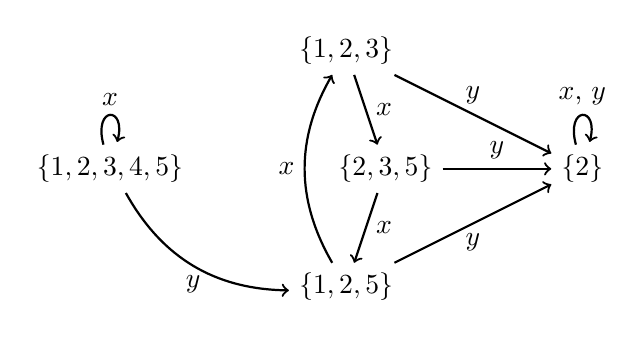
\begin{tikzpicture}[->,thick]
      \node (1)  at (0,   1.5) {$\{1,2,3,4,5\}$};
      \node (2)  at (3,   3)   {$\{1,2,3\}$};
      \node (3)  at (3.5, 1.5) {$\{2,3,5\}$};
      \node (4)  at (3,   0)   {$\{1,2,5\}$};
      \node (5)  at (6,   1.5) {$\{2\}$};

      \path
        (1) edge [loop above] node {$x$} (1)
            edge [bend right] node [below] {$y$} (4)
        (2) edge node [right] {$x$} (3)
            edge node [above] {$y$} (5)
        (3) edge node [right] {$x$} (4)
            edge node [above] {$y$} (5)
        (4) edge [bend left] node [left] {$x$} (2)
            edge node [below] {$y$} (5)
        (5) edge [loop above] node {$x$, $y$} (5);
    \end{tikzpicture}
  \end{center}
  Roughly:
  \begin{itemize}
    \item
      $x \mathscr{R} y$ if $\ker(x) = \ker(y)$ and $\textrm{im}(x) \sim
      \textrm{im}(y)$ \emph{(plus group theory)}.
    \item
      $x \mathscr{L} y$ if $\textrm{im}(x) = \textrm{im}(y)$ and $\ker(x) \sim
      \ker(y)$ \emph{(plus group theory)}.
  \end{itemize}

  \vspace{1em}

  If there are fewer kernels/images than elements: net win!

  \emph{(Note: this structure also allows us to count idempotents.)}
}


% Slide: links to the Semigroups and Digraphs package
\frame{\frametitle{Semigroups and Digraphs packages for GAP}

  \begin{itemize}
    \item
      Semigroups package, version 2.8.0:\\
      {\color{blue}\url{gap-packages.github.io/Semigroups}}
  \end{itemize}

  \begin{itemize}
    \item
      Digraphs package, version 0.5.2:\\
      {\color{blue}\url{gap-packages.github.io/Digraphs}}
  \end{itemize}
}

\end{document}
